% !TeX encoding = UTF-8

\chapter{MATERIAIS E MÉTODOS}\label{ch:materiais-metodos}
Conforme mencionado anteriormente, o objetivo principal dessa dissertação é especificar e aplicar um modelo de RNA para análise e predição de valores acionários. Neste capítulo será realizada a pergunta de pesquisa e dos objetivos do trabalho na escolha da metodologia. Em seguida, esta metodologia será descrita e classificada quanto ao seu conteúdo e quanto aos métodos empregados na coleta e análise de dados.

\section{IDENTIFICAÇÃO DA PESQUISA}

Para se escolher a metodologia de pesquisa, alguns aspectos importantes precisaram ser analisados. Uma pesquisa pode ser realizada com dados criados ou com dados existentes. No primeiro caso, os dados são coletados após uma intervenção destinada a provocar uma mudança. No segundo, os dados estão presentes na situação em estudo e o pesquisador, por meio das técnicas de pesquisa, faz tais dados aparecerem, sem a intenção de modificá-los, através de uma intervenção. Na pesquisa experimental, delimita-se o fenômeno, formulam-se hipóteses, determinam-se os métodos e submete-se o fenômeno à experimentação em condições de controle \cite{laville}.

A escolha de uma estratégia de pesquisa tem que ser feita considerando-se, entre outros elementos, a natureza da questão da pesquisa, o contexto no qual a pesquisa se realizará, a formação e a experiência do pesquisador. De maneira geral, pode-se dividir as pesquisas em quantitativas ou experimentais e qualitativas \cite{laville}.

Ou seja, de acordo com as afirmativas acima, a presente pesquisa é caracterizada por ser experimental e qualitativa. Segundo \citeonline{chizzotti}, na pesquisa experimental, o pesquisador parte de um estado delimitado a priori, sobre qual cria possíveis hipóteses que podem ser analisadas, determinando os métodos de verificação a serem utilizados, através dos quais procurará controlar as condições do experimento.

\section{SELEÇÃO DAS AÇÕES}
Para iniciar o processo de desenvolvimento deste trabalho, é necessário definir quais ações serão escolhidas para compor a implementação. Os critérios para definir quais serão selecionadas, são caracterizados pelo alto potencial de movimentação e lucratividade na NASDAQ. Ou seja, são as empresas que mais influênciam na ecônomia, que, por coincidência, são do ramo da tecnologia \cite{christie}.

Tendo em vista os critérios especificados acima, as empresas selecionadas e o código de suas ações para a realização da coleta dos dados são:
\begin{itemize}
	\item Apple (AAPL);
	\item Amazon (AMZN);
	\item Cisco Systems (CSCO);
	\item Intel (INTC);
	\item Microsoft (MSFT);
\end{itemize}

\section{TÉCNICA PARA COLETA DE DADOS}
Com a definição da bolsa de valores em questão e das empresas que serão utilizadas para realizar a implementação deste trabalho, a próxima etapa se dá pela necessidade em coletar seus dados histórios.

Como os dados históricos das ações caracterizam-se por serem séries temporais, o tipo de técnica aplicada para conseguir indicadores de relevância para uma boa análise dos objetivos propostos, refere-se à análise técnica. 

Portanto, esta fase de coleta de dados é muito importante para o bom funcionamento da RNA que será criada, tornando-se essencial para o êxito final do trabalho.

\subsection{Definição das séries}
Selecionar os dados corretos para trabalhar com RNAs é uma fase de grande relevância, pois são esses dados que serão treinados e que irão garantir a estabilidade e a capacidade de generalização da rede em sí.

Sendo assim, a partir do conhecimento concebido pelo Capítulo 3, pode-se destacar dois aspectos importantes para a análise de quais dados coletar dentro de um problema em geral, sendo eles:

\begin{enumerate}
\item Dados que influeciam diretamente no resultado final e na coêrencia da análise proposta;
\item Uso de múltiplas séries de um mesmo dado para que a rede não se sujeite à \textit{overfitting} ou \textit{underfitting}.
\end{enumerate}

Segundo \citeonline{tororadar}, as variáveis que influenciam em um sistema de análise técnica das ações são:

\begin{enumerate}
\item Abertura: Valor da ação no ínicio do dia;
\item Máximo: Valor máximo negociado no dia;
\item Mínimo: Valor mínimo negociado no dia;
\item Volume: Número de negociações do papel no dia (valor bruto das negociações);
\item Valor de fechamento no dia;
\item Médias móveis simples: As médias móveis suavizam os dados de preços para formar um indicador de tendência sequencial. Elas não prevêem a direção dos preços, mas, antes, definem a sua direção atual com um atraso. Como o próprio nome indica, uma média móvel é uma média que se move. Os dados antigos são retirados, a medida que dados mais recentes se tornam disponíveis, isto faz com que a média se mova ao longo do tempo. A maioria das médias móveis são baseadas em preços de fechamento;
\item \textit{Moving Average Convergence Divergence} (MACD): indicador que controle a divergência e convergência das médias móveis. o MACD é formado pela diferença entre duas médias móveis, sendo uma de longo prazo e outra de curto prazo. Para o presente trabalho será calculado o MACD referente às médias de 26 e 10 dias.
\end{enumerate}

\section{FERRAMENTAS PARA COLETA DE DADOS}
Com a especificação das séries que serão coletadas, é necessário preparar um ambiente que dispõe o acesso à esses dados de forma simplificada. 

Pensando nesse contexto, é essencial utilizar uma linguagem de programação que tenha suporte à esse modelo de busca por dados. Tendo em vista essa premissa, a disponibilidade de uma API ou biblioteca é de extrema importância para a automatização deste processo.

\subsection{Linguagem de programação Python}
Segundo \citeonline{python-science}, apesar das diversas linguagens de programação disponíveis hoje para o desenvolvimento de aplicações e \textit{scripts}, a linguagem de programação Python vêm se destacando e crescendo constantemente na comunidade científica, seja por sua variedade de bibliotecas que auxiliam os desenvolvedores e pesquisadores à resolverem seus problemas de forma mais simplificada, até seu poder computacional e suas características de multiplataforma e multiparadigma.

Um fator que determina a utilização da linguagem de programação Python, como dito no paragrafo anterior, se dá pela sua variabilidade de bibliotecas voltadas, principalmente, para a análise de dados. Colocando isso no contexto deste trabalho, é essencial o uso de uma ferramenta que proporcione um alto nível de funcionalidades disponíveis para serem exploradas.

\subsection{Biblioteca pandas}\label{pandas-lib}
A biblioteca pandas é um pacote disponível na linguagem de programação Python que fornece fácil acesso à dados disponíveis na internet. O objetivo principal do pandas é justamente fornecer buscas flexíveis e intuítivas para a análise de dados estruturados e não estruturados. A biblioteca tem como objetivo específico se tornar a ferramenta de análise, busca e manipulação de dados aberta mais poderosa e flexível existente \cite{pandas}.

Segundo \citeonline{pandas}, o seu uso é adequado para diferentes tipos de dados, sendo eles:
\begin{enumerate}
\item Dados tabulares com colunas, como em uma tabela \textit{Structured Query Language} (SQL) de um banco de dados relacional ou uma planilha do Excel;
\item Dados de séries temporais não ordenados;
\item Qualquer outra forma de conjuntos de dados observacionais e estatísticos.
\end{enumerate}

Portanto, a principal justificativa para a utilização da biblioteca se dá pelo seu desenvolvimento, de código aberto, que impulsiona a comunidade a realizar diferentes aplicações, além da sua excelente documentação e suporte de acesso aos dados históricos da bolsa de valores NASDAQ, que são requisitos para a realização deste trabalho.

Para exemplificar como a biblioteca facilita o processo de coleta dos dados, o Código 2 ilustra uma pesquisa das ações da Microsoft, no período de 05/03/2001 a 11/04/2001.
\codigoPython\
\lstinputlisting[label=cod:script-coleta-dados, caption=\textit{Script} para coleta de dados]{src/microsoft.py}

As séries históricas são disponibilizadas em arquivos com valores separados por vírgulas (*.csv) contendo a data de negociação, valor de abertura, valores máximo e mínimo atingidos, valor de fechamento e o volume de negociações.

Na Figura 10 é possível observar o arquivo criado a partir do Código 2, demonstrando o formato especificado acima que a API retorna para a manipulação.

\begin{figure}[h]
	\centering
	\fbox{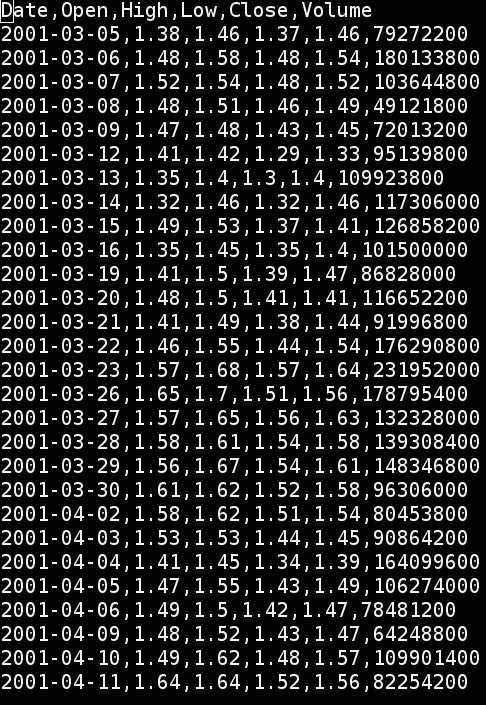
\includegraphics[width=0.5\textwidth, height=0.33\textheight]{dados-pandas}}
	\caption{Representação dos dados coletados pela biblioteca pandas}
	\fonte{Elaborado pelo autor}
	\label{exec-coleta-dados}
\end{figure}

\subsection{Google \textit{Finance} API}
É importante citar qual a fonte onde o pandas busca as séries históricas, por questões como confiabilidade dos dados. O acesso é realizado através da integração com o Google \textit{Finance} API, um banco de dados quase em tempo real mantido pelo Google, que trabalha com as principais bolsas de valores do mundo \cite{pandas}.

A API trabalha com um limite inicial para a coleta das ações, este limite se inicia em 03/05/2001 e vai se atualizando diariamente. Tendo em vista que para trabalhar com RNAs é importante buscar o máximo de informações possíveis e também considerando o limite disponível pela API, o período das ações das empresas selecionadas serão coletadas iniciando no ano de 2001 até o ano de 2017. 

Sendo assim, a ideia é preparar um ambiente que proporcione o uso dessa ferramenta, junto à biblioteca citada na \autoref{pandas-lib} para realizar a busca pelos dados necessários.

\subsection{PyCharm IDE}
É necessário utilizar uma \textit{Integrated Development Environment} (IDE) para auxiliar no \textit{script} de coleta de dados. PyCharm é uma IDE proprietária do grupo JetBrains que conta com uma versão livre para estudantes, que será realizada neste trabalho.
 
PyCharm suporta o desenvolvimento com a linguagem de programação Python desde a sua versão 2.4 até a versão 3.6. Vale citar que outras IDEs para o desenvolvimento poderiam ser utilizadas, porém a praticidade e a boa documentação das ferramentas JetBrains são fatores que justificam a sua utilização \cite{pycharm}.

\section{ESPECIFICAÇÃO DO MODELO DE REDES NEURAIS ARTIFICIAIS}\label{especifica-modelo}
Tendo como base o conhecimento adquirido no Capítulo 3, a definição de um modelo de RNA varia muito, sendo específico para cada problema do mundo real. Por isso, é importante frisar que não existe um modelo pré-definido e eficiente em RNAs, ficando a cargo da análise dos resultados, e, muitas vezes, por métodos de tentativa e erro para se chegar à um resultado eficiente \cite{haykin2000}.
 
Porém, com o estudo realizado no Capítulo 3, esse processo pode ser menos custoso do que parece. Avaliar o problema em que se está trabalhando junto com o conhecimento teórico é de grande auxílio para a especificação e construção de um modelo inicial que se aproxime do desejado.

Para especificar quais modelos não devem ser aplicados, ou seja, modelos que não tenham características referente a resolução do problema em questão, algumas perguntas-chave serão elaboradas, sendo elas:

\begin{enumerate}\label{enumerate-questions}
\item "Qual o modelo de dados se está trabalhando?";
\item "Estes dados serão treinados a partir de resultados esperados?";
\item "A RNA será exposta à uma quantidade significativa de dados desconhecidos aos treinados?".
\end{enumerate}

A primeira pergunta refere-se ao modelo de transmissão dos dados que a RNA deve implementar. Ou seja, se ela será formada por camadas adiante ou recorrente. Como é necessário o ajuste dos pesos nas camadas intermediárias, após a saída, a RNA deverá trabalhar com um modelo de camadas recorrente.

A segunda pergunta refere-se ao processo de aprendizagem. Se os dados são treinados com resultados esperados, a RNA deve possuir um método de aprendizado supervisionado, caso contrário, um modelo de RNA com treinamento não supervisionado deve ser utilizado. A RNA será treinada a partir dos resultados esperados através das séries temporais, ou seja, o modelo trabalhará com aprendizagem supervisionada.

A terceira pergunta refere-se à capacidade de generalização. Sendo assim, um modelo de RNA que irá trabalhar com dados desconhecidos deve ter caracteristícas de boa generalização, caso contrário, um modelo simples ja é o suficiente.

\subsection{Definição da Arquitetura}

Tendo em vista estes critérios estabelecidos na Seção anterior, chega-se a definição de que a RNA deverá possuir uma arquitetura de camadas recorrente, um método de aprendizado supervisionado e uma função de custo, para controlar o processo de generalização da mesma.

\citeonline{haykin2000} direciona este modelo de rede ao Perceptron de Múltiplas Camadas (MLP, \textit{Multilayer Perceptron}), são redes neurais compostas por um conjunto de unidades sensoriais que constituem a camada de entrada, uma ou mais camadas ocultas e uma camada de saída, onde o sinal de entrada se propaga para frente através da rede, camada por camada. Redes MLP trabalham normalmente junto ao algoritmo \textit{backproagation} para realizar seu treinamento e aprendizado.